\documentclass[11pt]{charter}

% El títulos de la memoria, se usa en la carátula y se puede usar el cualquier lugar del documento con el comando \ttitle
\titulo{Estimación de la captura realizada en buques pesqueros mediante visión artificial} 

% Nombre del posgrado, se usa en la carátula y se puede usar el cualquier lugar del documento con el comando \degreename
%\posgrado{Carrera de Especialización en Sistemas Embebidos} 
%\posgrado{Carrera de Especialización en Inteligencia  de las Cosas} 
\posgrado{Carrera de Especialización en Inteligencia Artificial}
%\posgrado{Maestría en Sistemas Embebidos} 
%\posgrado{Maestría en Internet de las cosas}

% Tu nombre, se puede usar el cualquier lugar del documento con el comando \authorname
\autor{Lic. Nicolás Eduardo Horro} 

% El nombre del director y co-director, se puede usar el cualquier lugar del documento con el comando \supname y \cosupname y \pertesupname y \pertecosupname
\director{Dr. Félix Ramón Rojo}
\pertenenciaDirector{INVAP S.E.} 
% FIXME:NO IMPLEMENTADO EL CODIRECTOR ni su pertenencia
%\codirector{} % si queda vacio no se deberíá incluir 
%\pertenenciaCoDirector{}

% Nombre del cliente, quien va a aprobar los resultados del proyecto, se puede usar con el comando \clientename y \empclientename
\cliente{Dr. Jorge Omar Lugo}
\empresaCliente{INVAP S.E.}

% Nombre y pertenencia de los jurados, se pueden usar el cualquier lugar del documento con el comando \jurunoname, \jurdosname y \jurtresname y \perteunoname, \pertedosname y \pertetresname.
\juradoUno{Nombre y Apellido (1)}
\pertenenciaJurUno{pertenencia (1)} 
\juradoDos{Nombre y Apellido (2)}
\pertenenciaJurDos{pertenencia (2)}
\juradoTres{Nombre y Apellido (3)}
\pertenenciaJurTres{pertenencia (3)}
 
\fechaINICIO{05 de agosto de 2021}		%Fecha de inicio de la cursada de GdP \fechaInicioName
\fechaFINALPlanificacion{13 de marzo de 2021} 	%Fecha de final de cursada de GdP
\fechaFINALTrabajo{23 de abril de 2021}		%Fecha de defensa pública del trabajo final


\begin{document}

\maketitle
\thispagestyle{empty}
\pagebreak


\thispagestyle{empty}
{\setlength{\parskip}{0pt}
\tableofcontents{}
}
\pagebreak


\section{Registros de cambios}
\label{sec:registro}


\begin{table}[ht]
\label{tab:registro}
\centering
\begin{tabularx}{\linewidth}{@{}|c|X|c|@{}}
\hline
\rowcolor[HTML]{C0C0C0} 
Revisión & \multicolumn{1}{c|}{\cellcolor[HTML]{C0C0C0}Detalles de los cambios realizados} & Fecha      \\ \hline
1.0      & Creación del documento                                          & 05/03/2021 \\ \hline
1.1      & Avances en alguna cosa                                          & dd/mm/aaaa \\ \hline
1.2      & Otro ejemplo \newline
		   Con texto partido \newline
		   En varias líneas \newline
		   A propósito                                                     & dd/mm/aaaa \\ \hline
\end{tabularx}
\end{table}

\pagebreak

\section{Acta de constitución del proyecto}
\label{sec:acta}

\begin{flushright}
San Carlos de Bariloche, \fechaInicioName
\end{flushright}

\vspace{2cm}

Por medio de la presente se acuerda con el Lic. \authorname\hspace{1px} que su Trabajo Final de la \degreename\hspace{1px} se titulará ``\ttitle'', consistirá esencialmente en el prototipo preliminar de un sistema para clasificación de capturas y descarte en buques pesqueros utilizando técnicas visión por computadora e inteligencia artificial, y tendrá un presupuesto preliminar estimado de 600 hs de trabajo, con fecha de inicio \fechaInicioName\hspace{1px} y fecha de presentación pública \fechaFinalName.

Se adjunta a esta acta la planificación inicial.

\vfill

% Esta parte se construye sola con la información que hayan cargado en el preámbulo del documento y no debe modificarla
\begin{table}[ht]
\centering
\begin{tabular}{ccc}
\begin{tabular}[c]{@{}c@{}}Ariel Lutenberg \\ Director posgrado FIUBA\end{tabular} & \hspace{2cm} & \begin{tabular}[c]{@{}c@{}}\clientename \\ \empclientename \end{tabular} \vspace{2.5cm} \\ 
\multicolumn{3}{c}{\begin{tabular}[c]{@{}c@{}} \supname \\ Director del Trabajo Final\end{tabular}} \vspace{2.5cm} \\
%\begin{tabular}[c]{@{}c@{}}\jurunoname \\ Jurado del Trabajo Final\end{tabular}     &  & \begin{tabular}[c]{@{}c@{}}\jurdosname\\ Jurado del Trabajo Final\end{tabular}  \vspace{2.5cm}  \\
%\multicolumn{3}{c}{\begin{tabular}[c]{@{}c@{}} \jurtresname\\ Jurado del Trabajo Final\end{tabular}} \vspace{.5cm}                                                                     
\end{tabular}
\end{table}

\section{Descripción técnica-conceptual del proyecto a realizar}
\label{sec:descripcion}

\begin{consigna}{red}
El objetivo es que el lector en una o dos páginas entienda de qué se trata el proyecto y cuáles son sus desafíos, su motivación y su importancia.
Se debe destacar claramente cuál es el valor que agrega el proyecto a realizar. ``El presente proyecto se destaca especialmente por incorporar tal cosa... Esto lo diferencia de otros sistemas similares en que ...''

Puede ser útil incluir en esta sección la respuesta a alguna de estas preguntas:

\begin{itemize}
\item ¿Cómo se vincula este proyecto con la misión de la organización?
\item ¿Cómo se inserta este proyecto en el modelo de negocio de la organización?
\item ¿Ayuda a la explicación si se incluye un lienzo Canvas del Modelo de Negocio?
\item ¿En qué estado del ciclo de vida está el producto que se desea reemplazar o mejorar?
\item ¿Cuales son las necesidades que debe satisfacer?
\item ¿Por dónde pasa la innovación?
\end{itemize}

La descripción técnica-conceptual \textbf{debe incluir al menos un diagrama en bloques del sistema }y una frase como la siguiente: ``En la Figura \ref{fig:diagBloques} se presenta el diagrama en bloques del sistema. Se observa que...''. Luego recién más abajo de haber puesto esta frase se pone la figura. La regla es que las figuras nunca pueden ir antes de ser mencionadas en el texto, porque sino el lector no entiende por qué de pronto aparece una figura.

\vspace{25px}

\begin{figure}[htpb]
\centering 
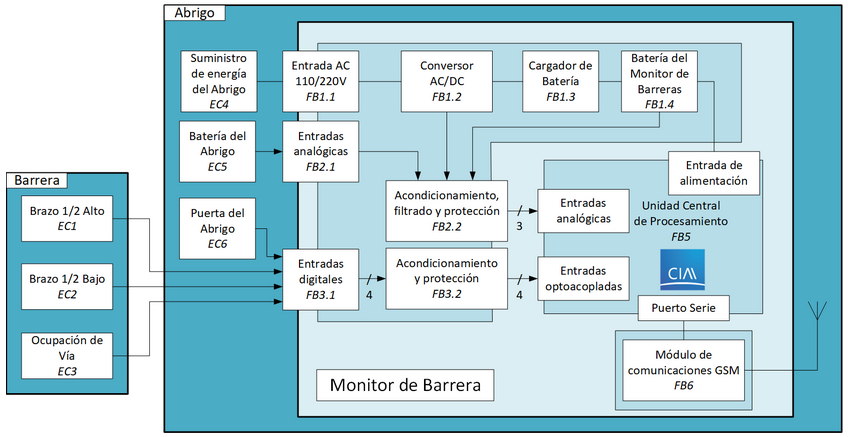
\includegraphics[width=.7\textwidth]{./Figuras/diagBloques.png}
\caption{Diagrama en bloques del sistema}
\label{fig:diagBloques}
\end{figure}

\vspace{25px}

El tamaño de la tipografía en la figura debe ser adecuado para que NO pase lo que ocurre acá, donde el lector debe esforzarse para poder leer el texto. Los colores usados en el diagrama deben ser adecuados, tal que ayuden a comprender mejor el diagrama.
\end{consigna}

% Recordar borrar consigna!
El presente proyecto consiste en un prototipo que extiende el Sistema de Monitoreo Electrónico (SME) en los sistemas de Circuitos Cerrados de Televisión (CCTV) a bordo de los buques pesqueros mediante el uso Inteligencia Artificial (IA). El objetivo es la clasificación y estimación de cantidad de las piezas capturadas y descartadas, proceso que actualmente se realiza de manera manual y resulta costoso y propenso a errores. 

\subsection{Introducción general al tema}

La pesca industrial es un tipo de pesca que tiene como objetivo obtener un gran número de capturas. En Argentina el sector primario pesquero (aquél que se ocupa de la captura) se compone de una flota de buques fresqueros de altura, de costeros grandes y costeros chicos y una flota de buques procesadores. La flota fresquera de altura está conformada por barcos arrastreros con bodegas refrigeradas y cuentan con equipamiento de navegación y detección y utilizan redes de arrastre.

La figura \ref{fig:tipo_embarcaciones} expone un diagrama simplificado de los tipos de embarcaciones y métodos de captura de acuerdo a la profundidad.

\vspace{25px}

\begin{figure}[htpb]
\centering 
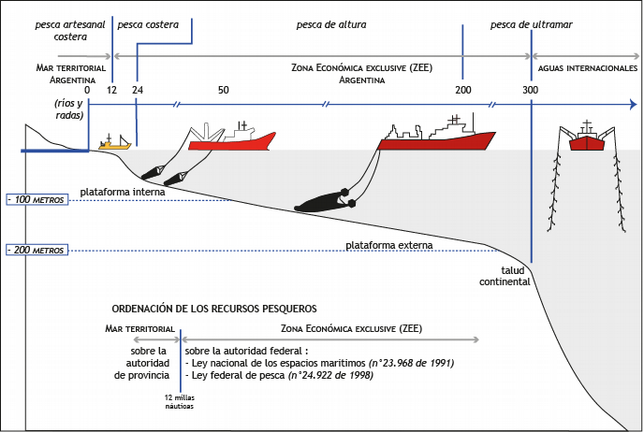
\includegraphics[width=.7\textwidth]{./Figuras/tipo_embarcaciones.png}
\caption{Tipos de embarcaciones según el tipo de pesca}
\label{fig:tipo_embarcaciones}
\end{figure}

\vspace{25px}

A fin de garantizar que la pesca a esta escala sea sostenible, el Consejo Federal Pesquero tiene como funciones el establecimiento de la política pesquera y de la política de investigación pesquera nacional, la planificación del desarrollo pesquero nacional, el establecimiento de la Captura Máxima Permisible (CMP) por especie y las cuotas de captura, así como aprobar los permisos de pesca comercial y experimental y fijar los cánones por el ejercicio de la pesca, entre otros. 
Dado que una pesquería es un sistema complejo de factores interdependientes entre los que se cuentan el estado del recurso biológico, limitaciones sociales e institucionales, condiciones económicas y convicciones culturales, etc- es importante generar información estadística e indicadores que permitan el análisis de la actividad de las pesquerías para poder establecer de manera precisa su marco regulatorio.
El monitoreo y la vigilancia deben permitir conocer las características del esfuerzo en la actividad pesquera y asegurar que las capturan se realicen dentro de los cánones admitidos. Existen también regulaciones que establecen el modo en que debe emplearse la técnica, por ejemplo, exigiendo una permanencia mínima de las redes en el fondo para disminuir la captura incidental de mamíferos marinos.
Tradicionalmente, la principal manera de recopilar información independiente acerca de las actividades y la captura de los buques ha sido mediante observadores a bordo, pero existe una creciente tendencia a la utilización de sistemas electrónicos y un mayor grado de automatización.
El Seguimiento Electrónico (EM) se presenta como una alternativa eficiente y rentable.
Si bien el registro y monitoreo digital de las actividades a bordo representa un avance respecto a la elaboración de reportes manuscritos, el análisis de la cantidad datos generados, la manipulación de sus medios de almacenamiento y la dependencia de observadores calificados para su análisis, no deja de ser una alternativa costosa y también propensa a otro tipo de errores.

La figura \ref{fig:seguimiento_electronico} muestra un esquema de un sistema de seguimiento electrónico típico y algunos ejemplos de sus usos.

\vspace{25px}

\begin{figure}[htpb]
\centering 
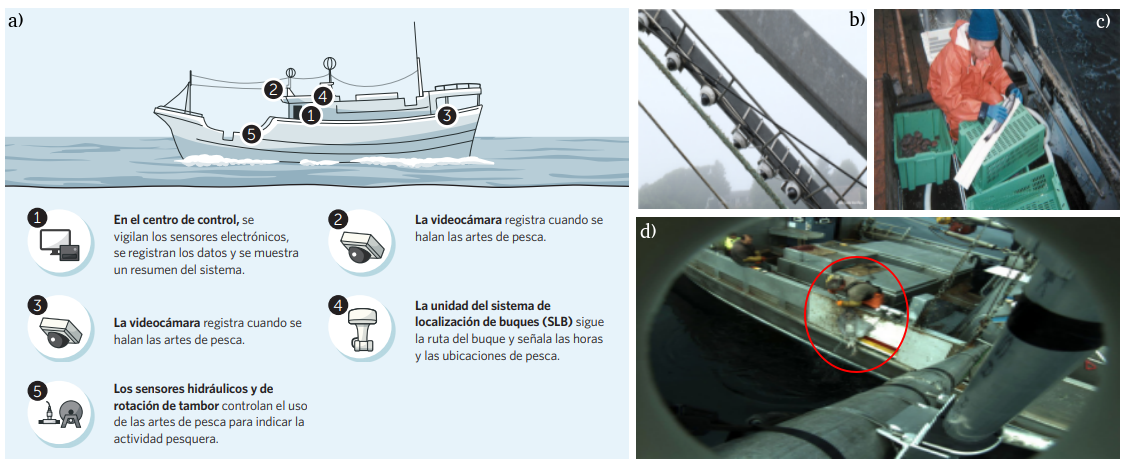
\includegraphics[width=.7\textwidth]{./Figuras/seguimiento_electronico.png}
\caption{ a) Sistema de Seguimiento Electrónico. b) Sistema de CCTV apuntando a redes de arrastre. c) Registro de especímenes por observadores calificados. d) Cámara captando descarte de especie protegida, probablemente no declarada.}
\label{fig:seguimiento_electronico}
\end{figure}

\vspace{25px}

Las nuevas técnicas en las áreas de Visión por Computadora e Inteligencia Artificial hallan un posible campo de aplicación en la optimización de estas tareas de análisis, como lo demuestran algunos trabajos con resultados alentadores. Por otra parte, el conocido sitio de competencias de aprendizaje automático Kaggle realizó una competencia de clasificación de capturas en buques pesqueros también con el tema de  combatir la sobreexplotación del recurso.

\subsection{Marco de la propuesta}

INVAP S.E. es una empresa del Gobierno de Río Negro dedicada al diseño y construcción de sistemas tecnológicos complejos, con una trayectoria de cuatro décadas en el mercado nacional y tres en la escena internacional. La empresa define como su misión el desarrollo de tecnología de avanzada en diferentes campos de la industria, la ciencia y la investigación aplicada, creando “paquetes tecnológicos” de alto valor agregado tanto para satisfacer necesidades nacionales como para insertarse en mercados externos a través de la exportación.
Dentro del contexto de la búsqueda de nuevos negocios e incorporación de nuevas tecnologías, se realizan trabajos de investigación y prototipos, a menudo mediante convenios con universidades y otras organizaciones, ya sea en calidad de pasantías, prácticas profesionales, trabajos de carreras de grado y posgrado, u otros. Estos trabajos pueden eventualmente evolucionar y aprovecharse en un proyecto de mayor envergadura.
El proyecto que se describe es uno de estos casos y se integra en un desarrollo de mayor alcance: un sistema que utiliza cámaras de video y computadoras o dispositivos auxiliares para el control de la pesca que incorpora gradualmente mayores niveles de automatismo y capacidades de reporte en tiempo real. 
El principal cliente interesado es el Estado Argentino, y en particular la Subsecretaría de Pesca y Acuicultura perteneciente a la Secretaría de Agricultura, Ganadería y Pesca del Ministerio de Agricultura, Ganadería y Pesca. Si bien no son clientes directos, es también importante mencionar la participación del Consejo Federal Pesquero (https://cfp.gob.ar/) y de INIDEP(https://www.argentina.gob.ar/inidep)), organismos involucrados en el seguimiento y regulación de la explotación del recurso y promotores de la modernización de los sistemas de monitoreo y seguimiento. También pueden ser potenciales usuarios centros de investigación o entes privados que lo utilicen para registro propio. El desarrollo y vinculación con instituciones se realiza por medio de INVAP S.E y para este trabajo representa la aceptación técnica por parte del cliente el Dr. Jorge Omar Lugo.
Como se mencionó, este trabajo es un subproducto de un proyecto de mayor envergadura. El desarrollo actual de INVAP S.E. tiene como objetivos posibilitar el registro de video y de otros dispositivos (por ejemplo motores de las redes de arrastre) para su posterior análisis en tierra (dependiendo del caso puede ser hasta luego de 30 días en el mar), la segunda etapa es el procesamiento y envío del parte de pesca en tiempo real, y por último la automatización de algunas tareas de análisis. Este trabajo es un prototipo para la tercer etapa. 


\subsection{Descripción del proyecto}

La distorsión de lente de pez que suelen tener las cámaras de vigilancia, las condiciones de iluminación variables (zonas de escaso contraste por la fuerte saturación de luces fluorescentes y otras casi sin iluminar) y la dificultad para detectar una estructura por la forma y disposición de las presas hacen que resulte difícil garantizar una correcta detección por un método automático.

La figura \ref{fig:ejemplos_escenas} muestra ejemplos de los tipos de escenas en las cuales se apunta a realizar la detección.

\vspace{25px}

\begin{figure}[htpb]
\centering 
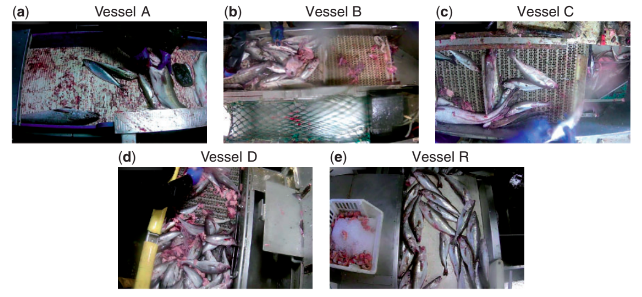
\includegraphics[width=.7\textwidth]{./Figuras/ejemplos_escenas.png}
\caption{Comparación de imágenes de cámaras en distintos buques. La orientación aleatoria de las presas y su mutua oclusión, y la difícil estructura de la escena presentan un desafío para los algoritmos de detección}
\label{fig:ejemplos_escenas}
\end{figure}

\vspace{25px}

Aún así, la literatura consultada y las soluciones con mejor desempeño presentadas en muestran que se pueden obtener resultados aceptables utilizando alguna variante de red convolucional (CNN, por sus siglas en inglés Convolutional Neural Network). 
Una característica de las redes neuronales profundas es que requieren una gran cantidad de datos de entrenamiento, que en este caso (a diferencia de como ocurre en otros dominios, como el reconocimiento de personas, caras, vehículos, carteles, etc.) es difícil (o costoso) obtener.

La innovación de esta propuesta reside en la aplicación del estado del arte de estas técnicas a un dominio para el cuál no existen productos o soluciones en el mercado.

Se propone una solución integrada por los siguientes bloques:

Ingesta de Video: obtiene la los cuadros de una cámara o un archivo de video y aplica una corrección de imagen para reducir las diferencias entre cámaras. Esta corrección puede incluir: contrarrestar distorsión de lente de pez, aplicar transformaciones de coordenadas cromáticas, ecualizar la imagen, etc.

Detección: este bloque recibe los cuadros de video procesados de la etapa anterior y por cada cuadro extrae las regiones de interés y la probabilidad de que exista alguna de las clases detectadas. Se utilizará el algoritmo YOLOv4 o variantes del mismo, dado que representa el estado del arte y es apto para procesamiento en tiempo real si se dispone del HW apropiado. A menudo la capacidad de detección de un objeto puede depender de su orientación, condiciones de oclusión, iluminación, etc. Es posible que un objeto que no sea fácilmente identificable en un cuadro de video, sí lo sea en otros cuadros de ese mismo video. Para este trabajo se propone usar un algoritmo de seguimiento que también representa el estado del arte, denominado DeepSORT. La salida de este algoritmo es una trayectoria de un objeto. Como etapa final, se propone un filtro para decidir si rechazar o no la detección y asociar un evento a esa trayectoria (por ejemplo, incrementar un contador de capturas, reportar un descarte, etc.).

Información de contexto (opcional): se puede utilizar información de localización del buque, fecha y hora, actividad de sistemas mecánicos y otros datos tanto para acompañar la salida del clasificador como para mejorarla, dado que hay especies que habitan determinados sectores o se capturan a determinada profundidade intervienen sistemas de captura específicos para un tipo de objetivo.

Registro y Generación de Reportes: la salida de la etapa anterior es registrada en una base de datos, para obtener trazabilidad de las capturas y descartes (horarios, tipos de capturas, cantidad de descartes, etc.). Para facilitar el consumo de esta información y permitir combinarla con otros servicios, se propone como interfaz un servicio REST sencillo que devuelve reportes para consultas típicas. Para la base de datos también se considerarán alternativas aptas para una implementación en un sistema embebido, por ejemplo [20,21]. Otra opción es utilizar InfluxDB [36] que ya incluye una interfaz de consulta y control REST, en cuyo caso se podría prescindir del servicio adicional.

La figura  \ref{fig:diagrama_bloques} muestra un diagrama de bloques de la solución propuesta.

\vspace{25px}

\begin{figure}[htpb]
\centering 
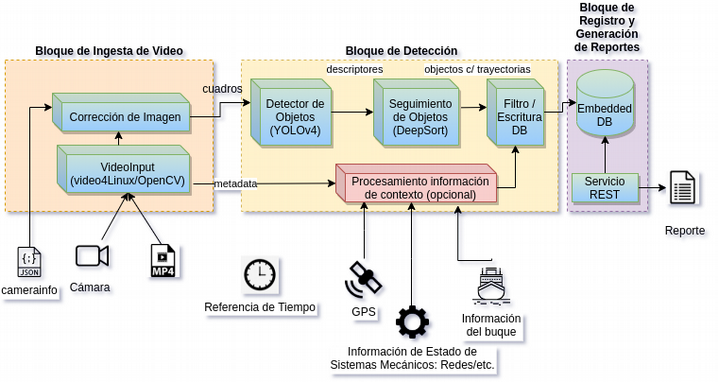
\includegraphics[width=.7\textwidth]{./Figuras/diagrama_bloques.png}
\caption{Diagrama en bloques del sistema}
\label{fig:diagrama_bloques}
\end{figure}

\vspace{25px}


\section{Identificación y análisis de los interesados}
\label{sec:interesados}

\begin{consigna}{red} 
Nota: (borrar esto y todas las consignas en color rojo antes de entregar este documento).
 
Es inusual que una misma persona esté en más de un rol, incluso en proyectos chicos.
 
Si se considera que una persona cumple dos o más roles, entonces sólo dejarla en el rol más importante. Por ejemplo:

\begin{itemize}
\item Si una persona es Cliente pero también colabora u orienta, dejarla solo como Cliente.
\item Si una persona es el Responsable, no debe ser colocado también como Miembro del equipo.
\end{itemize}

Pero en cambio sí es usual que el Cliente y el Auspiciante sean el mismo, por ejemplo.

\begin{table}[ht]
%\caption{Identificación de los interesados}
%\label{tab:interesados}
\begin{tabularx}{\linewidth}{@{}|l|X|X|l|@{}}
\hline
\rowcolor[HTML]{C0C0C0} 
Rol           & Nombre y Apellido & Organización 	& Puesto 	\\ \hline
Cliente       & \clientename      &\empclientename	& -       	\\ \hline
Responsable   & \authorname       & FIUBA        	& Alumno 	\\ \hline
Orientador    & \supname	      & \pertesupname 	& Director	Trabajo final \\ \hline
\end{tabularx}
\end{table}

El Director suele ser uno de los Orientadores.

No dejar celdas vacías; si no hay nada que poner en una celda colocar un signo ``-''.

No dejar filas vacías; si no hay nada que poner en una fila entonces eliminarla.

Sería deseable listar a continuación de la tabla las principales características de cada interesado.
 
Por ejemplo:
\begin{itemize}
\item Auspiciante: es riguroso y exigente con la rendición de gastos. Tener mucho cuidado con esto.
\item Equipo: Juan Perez, suele pedir licencia porque tiene un familiar con una enfermedad. Planificar considerando esto.
\item Orientador: María Gómez, nos va a poder ayudar mucho con la gestión de impuestos.
\end{itemize}

\end{consigna}

\section{1. Propósito del proyecto}
\label{sec:proposito}

\begin{consigna}{red}
¿Por qué se hace el proyecto? ¿Qué se quiere lograr? 

Se recomienda que sea solo un párrafo que empiece diciendo ``El propósito de este proyecto es...''.
\end{consigna}

El propósito de este proyecto es incorporar al proyecto del sistema de control de pesca que está siendo desarrollado por INVAP S.E. un componente adicional para la automatización de las tareas de registro e inspección.

\section{2. Alcance del proyecto}
\label{sec:alcance}

\begin{consigna}{red}
¿Qué se incluye y que no se incluye en este proyecto?

Se refiere al trabajo a hacer para entregar el producto o resultado especificado. 

Explicitar todo lo quede comprendido dentro del alcance del proyecto.

Explicitar además todo lo que no quede incluido (``El presente proyecto no incluye...'')

\end{consigna}

El presente proyecto contempla todo el software a desarrollar para el ciclo completo que se expuso en la figura \ref{fig:diagrama_bloques} desde la adquisición de una imagen (utilizando los drivers o formato de publicación de las cámaras) hasta el reporte almacenado en las bases de datos.


\section{3. Supuestos del proyecto}
\label{sec:supuestos}

\begin{consigna}{red}
``Para el desarrollo del presente proyecto se supone que: ...''

\begin{itemize}
\item Supuesto 1
\item Supuesto 2...
\end{itemize}

Por ejemplo, se podrían incluir supuestos respecto a disponibilidad de tiempo y recursos humanos y materiales, sobre la factibilidad técnica de distintos aspectos del proyecto, sobre otras cuestiones que sean necesarias para el éxito del proyecto como condiciones macroeconómicas o reglamentarias.
\end{consigna}

Para el desarrollo del presente proyecto se supone que:

\begin{itemize}
\item Se contará con los datos necesarios. Se recomienda para éstos contar con un mínimo de 2000 ejemplos por cada clase de objeto a detectar. Si no pudiera alcanzarse este número, existen técnicas para compensar la falta de datos, pero puede verse penalizado el desempeño final del algoritmo y su capacidad de generalizar, siendo necesario un trabajo de ingeniería de features dependiendo de las características de las escenas en los que se utilizará.
\item Contando con datos de cantidad y calidad suficiente, los algoritmos de la familia YOLOv4 y DeepSORT son aptos para resolver esta tarea con un desempeño igual o ligeramente superior al de un operador humano o de un mAP de 70\%.
\item Se contará con el HW disponible para desarrollo y ejecución del proyecto.
\end{itemize}

\section{4. Requerimientos}
\label{sec:requerimientos}

\begin{consigna}{red}
Los requerimientos deben numerarse y de ser posible agruparlos por afinidad:

\begin{enumerate}
\item Grupo de requerimientos asociados con...
	\begin{enumerate}
	\item Requerimiento 1
	\item Requerimiento 2
	\item Requerimiento 3 (prioridad menor)
	\end{enumerate}
\item Grupo de requerimientos asociados con...
	\begin{enumerate}
	\item Requerimiento 1
	\item Requerimiento 2 (prioridad menor)
	\end{enumerate}
\end{enumerate}

Leyendo los requerimientos se debe poder interpretar cómo será el proyecto y su funcionalidad.

De ser posible indicar cómo se obtuvieron cada uno de los requerimientos 

Indicar claramente cuál es la prioridad entre los distintos requerimientos. 

No olvidarse de que los requerimientos incluyen a las regulaciones y normas vigentes!!!

Y al escribirlos seguir las siguientes reglas:
\begin{itemize}
\item Ser breve y conciso (nadie lee cosas largas). 
\item Ser específico: no dejar lugar a confusiones.
\item Expresar los requerimientos en términos que sean cuantificables y medibles.
\end{itemize}

\end{consigna}

begin{enumerate}
\item Requerimientos generales
	\begin{enumerate}
	\item Requerimiento 1
	\item Requerimiento 2
	\item Requerimiento 3 (prioridad menor)
	\end{enumerate}
\item Requerimientos funcionales
	\begin{enumerate}
	\item Requerimiento 1
	\item Requerimiento 2 (prioridad menor)
	\end{enumerate}
\item Requerimientos de desempeño	
	\begin{enumerate}
	\item Requerimiento 1
	\item Requerimiento 2 (prioridad menor)
	\end{enumerate}
\item Requerimientos de interface
	\begin{enumerate}
	\item Requerimiento 1
	\item Requerimiento 2 (prioridad menor)
	\end{enumerate}	
\item Requerimientos de ambiente
	\begin{enumerate}
	\item Requerimiento 1
	\item Requerimiento 2 (prioridad menor)
	\end{enumerate}		
\item Restricciones de diseño
	\begin{enumerate}
	\item Requerimiento 1
	\item Requerimiento 2 (prioridad menor)
	\end{enumerate}	
\end{enumerate}

\section{Historias de usuarios (\textit{Product backlog})}
\label{sec:backlog}

\begin{consigna}{red}
Descripción: En esta sección se deben incluir las historias de usuarios y su ponderación (\textit{history points}). Recordar que las historias de usuarios son descripciones cortas y simples de una característica contada desde la perspectiva de la persona que desea la nueva capacidad, generalmente un usuario o cliente del sistema. La ponderación es un número entero que representa el tamaño de la historia comparada con otras historias de similar tipo.
\end{consigna}

\section{5. Entregables principales del proyecto}
\label{sec:entregables}

\begin{itemize}
\item Documento de Diseño
\item Manual de Usuario
\item Código fuente
\item Informe final
\end{itemize}

\section{6. Desglose del trabajo en tareas}
\label{sec:wbs}

\begin{consigna}{red}
Se recomienda mostrar el WBS mediante una lista indexada:

\begin{enumerate}
\item Grupo de tareas 1
	\begin{enumerate}
	\item Tarea 1 (tantas hs)
	\item Tarea 2 (tantas hs)
	\item Tarea 3 (tantas hs)
	\end{enumerate}
\item Grupo de tareas 2
	\begin{enumerate}
	\item Tarea 1 (tantas hs)
	\item Tarea 2 (tantas hs)
	\item Tarea 3 (tantas hs)
	\end{enumerate}
	\item Grupo de tareas 3
	\begin{enumerate}
	\item Tarea 1 (tantas hs)
	\item Tarea 2 (tantas hs)
	\item Tarea 3 (tantas hs)
	\item Tarea 4 (tantas hs)
	\item Tarea 5 (tantas hs)
	\end{enumerate}
\end{enumerate}

Cantidad total de horas: (tantas hs)

Se recomienda que no haya ninguna tarea que lleve más de 40 hs. 

\end{consigna}


\begin{enumerate}
\item Implementación de bloque de preprocesamiento
	\begin{enumerate}
	\item Tarea 1 (tantas hs)
	\item Tarea 2 (tantas hs)
	\item Tarea 3 (tantas hs)
	\item Tarea 4 (tantas hs)
	\item Tarea 5 (tantas hs)
	\end{enumerate}	
\item Implementación de bloque de detección
	\begin{enumerate}
	\item Tarea 1 (tantas hs)
	\item Tarea 2 (tantas hs)
	\item Tarea 3 (tantas hs)
	\end{enumerate}
\item Implementación de bloque de seguimiento
	\begin{enumerate}
	\item Tarea 1 (tantas hs)
	\item Tarea 2 (tantas hs)
	\item Tarea 3 (tantas hs)
	\end{enumerate}
\item Implementación de bloque de clasificación final
	\begin{enumerate}
	\item Tarea 1 (tantas hs)
	\item Tarea 2 (tantas hs)
	\item Tarea 3 (tantas hs)
	\item Tarea 4 (tantas hs)
	\item Tarea 5 (tantas hs)
	\end{enumerate}
\item Implementación de bloque de reporte/almacenamiento
	\begin{enumerate}
	\item Tarea 1 (tantas hs)
	\item Tarea 2 (tantas hs)
	\item Tarea 3 (tantas hs)
	\item Tarea 4 (tantas hs)
	\item Tarea 5 (tantas hs)
	\end{enumerate}	
\item Integración y documentación
	\begin{enumerate}
	\item Tarea 1 (tantas hs)
	\item Tarea 2 (tantas hs)
	\item Tarea 3 (tantas hs)
	\item Tarea 4 (tantas hs)
	\item Tarea 5 (tantas hs)
	\end{enumerate}		
\end{enumerate}

Cantidad total de horas: 640hs.

\section{7. Diagrama de Activity On Node}
\label{sec:AoN}

\begin{consigna}{red}
Armar el AoN a partir del WBS definido en la etapa anterior. 

%La figura \ref{fig:AoN} fue elaborada con el paquete latex tikz y pueden consultar la siguiente referencia \textit{online}:

%\url{https://www.overleaf.com/learn/latex/LaTeX_Graphics_using_TikZ:_A_Tutorial_for_Beginners_(Part_3)\%E2\%80\%94Creating_Flowcharts}

\end{consigna}

\begin{figure}[htpb]
\centering 
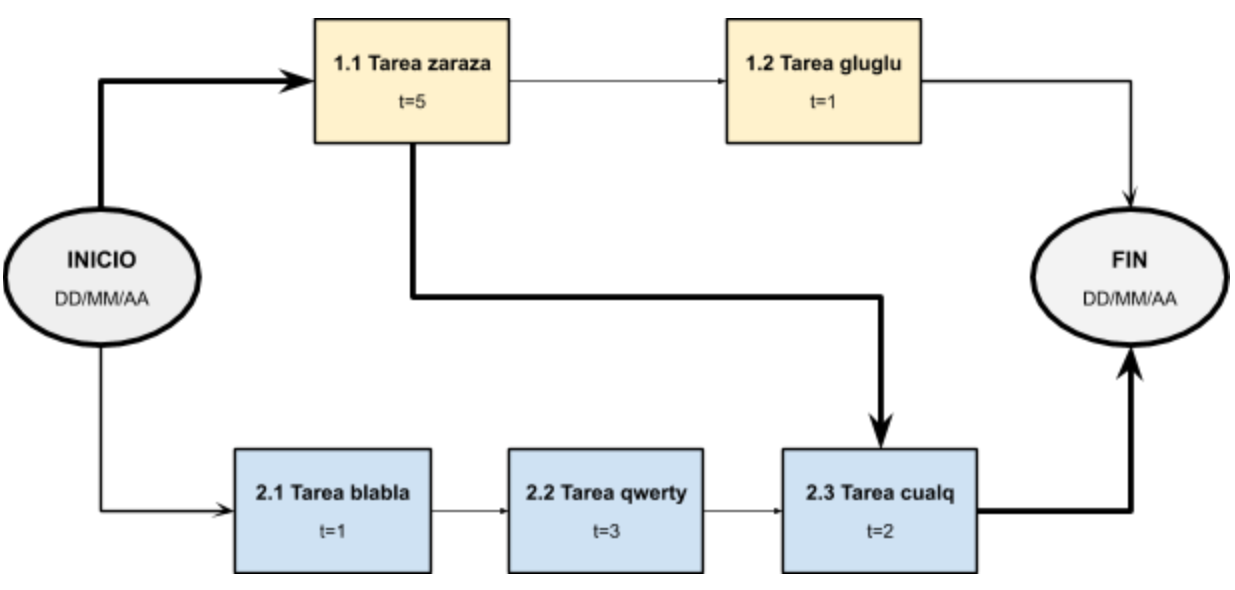
\includegraphics[width=.8\textwidth]{./Figuras/AoN.png}
\caption{Diagrama en \textit{Activity on Node}}
\label{fig:AoN}
\end{figure}

Indicar claramente en qué unidades están expresados los tiempos.
De ser necesario indicar los caminos semicríticos y analizar sus tiempos mediante un cuadro.
Es recomendable usar colores y un cuadro indicativo describiendo qué representa cada color, como se muestra en el siguiente ejemplo:



\section{8. Diagrama de Gantt}
\label{sec:gantt}

\begin{consigna}{red}
Utilizar el software Gantter for Google Drive o alguno similar para dibujar el diagrama de Gantt.

Existen muchos programas y recursos \textit{online} para hacer diagramas de gantt, entre las cuales destacamos:

\begin{itemize}
\item Planner
\item GanttProject
\item Trello + \textit{plugins}. En el siguiente link hay un tutorial oficial: \\ \url{https://blog.trello.com/es/diagrama-de-gantt-de-un-proyecto}
\item Creately, herramienta online colaborativa. \\\url{https://creately.com/diagram/example/ieb3p3ml/LaTeX}
\item Se puede hacer en latex con el paquete \textit{pgfgantt}\\ \url{http://ctan.dcc.uchile.cl/graphics/pgf/contrib/pgfgantt/pgfgantt.pdf}
\end{itemize}

Pegar acá una captura de pantalla del diagrama de Gantt, cuidando que la letra sea suficientemente grande como para ser legible. 
Si el diagrama queda demasiado ancho, se puede pegar primero la ``tabla'' del Gantt y luego pegar la parte del diagrama de barras del diagrama de Gantt.

Configurar el software para que en la parte de la tabla muestre los códigos del EDT (WBS).\\
Configurar el software para que al lado de cada barra muestre el nombre de cada tarea.\\
Revisar que la fecha de finalización coincida con lo indicado en el Acta Constitutiva.

En la figura \ref{fig:gantt}, se muestra un ejemplo de diagrama de gantt realizado con el paquete de \textit{pgfgantt}. En la plantilla pueden ver el código que lo genera y usarlo de base para construir el propio.

\begin{figure}[htbp]
\begin{center}
\begin{ganttchart}{1}{12}
  \gantttitle{2020}{12} \\
  \gantttitlelist{1,...,12}{1} \\
  \ganttgroup{Group 1}{1}{7} \\
  \ganttbar{Task 1}{1}{2} \\
  \ganttlinkedbar{Task 2}{3}{7} \ganttnewline
  \ganttmilestone{Milestone o hito}{7} \ganttnewline
  \ganttbar{Final Task}{8}{12}
  \ganttlink{elem2}{elem3}
  \ganttlink{elem3}{elem4}
\end{ganttchart}
\end{center}
\caption{Diagrama de gantt de ejemplo}
\label{fig:gantt}
\end{figure}

\end{consigna}

\section{9. Matriz de uso de recursos de materiales}
\label{sec:recursos}


\begin{table}
\label{tab:recursos}
\centering
\begin{tabularx}{\linewidth}{@{}|c|X|X|X|X|c|@{}}
\hline
\cellcolor[HTML]{C0C0C0} & \cellcolor[HTML]{C0C0C0} & \multicolumn{4}{c|}{\cellcolor[HTML]{C0C0C0}Recursos requeridos (horas)} \\ \cline{3-6} 
\multirow{-2}{*}{\cellcolor[HTML]{C0C0C0}\begin{tabular}[c]{@{}c@{}}Código\\ WBS\end{tabular}} & \multirow{-2}{*}{\cellcolor[HTML]{C0C0C0}\begin{tabular}[c]{@{}c@{}}Nombre \\ tarea\end{tabular}} & Material 1 & Material 2 & Material 3 & Material 4 \\ \hline
 &  &  &  &  &  \\ \hline
 &  &  &  &  &  \\ \hline
 &  &  &  &  &  \\ \hline
 &  &  &  &  &  \\ \hline
 &  &  &  &  &  \\ \hline
 &  &  &  &  &  \\ \hline
 &  &  &  &  &  \\ \hline
 &  &  &  &  &  \\ \hline 
 &  &  &  &  &  \\ \hline
 &  &  &  &  &  \\ \hline
 &  &  &  &  &  \\ \hline
 &  &  &  &  &  \\ \hline
 &  &  &  &  &  \\ \hline
 &  &  &  &  &  \\ \hline
 &  &  &  &  &  \\ \hline
 &  &  &  &  &  \\ \hline
 &  &  &  &  &  \\ \hline
 &  &  &  &  &  \\ \hline
 &  &  &  &  &  \\ \hline
 &  &  &  &  &  \\ \hline
 &  &  &  &  &  \\ \hline
 &  &  &  &  &  \\ \hline
 &  &  &  &  &  \\ \hline
 &  &  &  &  &  \\ \hline 
 &  &  &  &  &  \\ \hline
 &  &  &  &  &  \\ \hline
 &  &  &  &  &  \\ \hline
 &  &  &  &  &  \\ \hline

\end{tabularx}%
\end{table}


\section{10. Presupuesto detallado del proyecto}
\label{sec:presupuesto}

\begin{consigna}{red}
Si el proyecto es complejo entonces separarlo en partes:
\begin{itemize}
\item Un total global, indicando el subtotal acumulado por cada una de las áreas.
\item El desglose detallado del subtotal de cada una de las áreas.
\end{itemize}

IMPORTANTE: No olvidarse de considerar los COSTOS INDIRECTOS.

\end{consigna}

\begin{table}[htpb]
\centering
\begin{tabularx}{\linewidth}{@{}|X|c|r|r|@{}}
\hline
\rowcolor[HTML]{C0C0C0} 
\multicolumn{4}{|c|}{\cellcolor[HTML]{C0C0C0}COSTOS DIRECTOS} \\ \hline
\rowcolor[HTML]{C0C0C0} 
Descripción &
  \multicolumn{1}{c|}{\cellcolor[HTML]{C0C0C0}Cantidad} &
  \multicolumn{1}{c|}{\cellcolor[HTML]{C0C0C0}Valor unitario} &
  \multicolumn{1}{c|}{\cellcolor[HTML]{C0C0C0}Valor total} \\ \hline
 &
  \multicolumn{1}{c|}{} &
  \multicolumn{1}{c|}{} &
  \multicolumn{1}{c|}{} \\ \hline
 &
  \multicolumn{1}{c|}{} &
  \multicolumn{1}{c|}{} &
  \multicolumn{1}{c|}{} \\ \hline
\multicolumn{1}{|l|}{} &
   &
   &
   \\ \hline
\multicolumn{1}{|l|}{} &
   &
   &
   \\ \hline
\multicolumn{3}{|c|}{SUBTOTAL} &
  \multicolumn{1}{c|}{} \\ \hline
\rowcolor[HTML]{C0C0C0} 
\multicolumn{4}{|c|}{\cellcolor[HTML]{C0C0C0}COSTOS INDIRECTOS} \\ \hline
\rowcolor[HTML]{C0C0C0} 
Descripción &
  \multicolumn{1}{c|}{\cellcolor[HTML]{C0C0C0}Cantidad} &
  \multicolumn{1}{c|}{\cellcolor[HTML]{C0C0C0}Valor unitario} &
  \multicolumn{1}{c|}{\cellcolor[HTML]{C0C0C0}Valor total} \\ \hline
\multicolumn{1}{|l|}{} &
   &
   &
   \\ \hline
\multicolumn{1}{|l|}{} &
   &
   &
   \\ \hline
\multicolumn{1}{|l|}{} &
   &
   &
   \\ \hline
\multicolumn{3}{|c|}{SUBTOTAL} &
  \multicolumn{1}{c|}{} \\ \hline
\rowcolor[HTML]{C0C0C0}
\multicolumn{3}{|c|}{TOTAL} &
   \\ \hline
\end{tabularx}%
\end{table}


\section{11. Matriz de asignación de responsabilidades}
\label{sec:responsabilidades}
\begin{consigna}{red}
Establecer la matriz de asignación de responsabilidades y el manejo de la autoridad completando la siguiente tabla:

\begin{table}[htpb]
\centering
\resizebox{\textwidth}{!}{%
\begin{tabular}{|c|c|c|c|c|c|}
\hline
\rowcolor[HTML]{C0C0C0} 
\cellcolor[HTML]{C0C0C0} &
  \cellcolor[HTML]{C0C0C0} &
  \multicolumn{4}{c|}{\cellcolor[HTML]{C0C0C0}Listar todos los nombres y roles del proyecto} \\ \cline{3-6} 
\rowcolor[HTML]{C0C0C0} 
\cellcolor[HTML]{C0C0C0} &
  \cellcolor[HTML]{C0C0C0} &
  Responsable &
  Orientador &
  Equipo &
  Cliente \\ \cline{3-6} 
\rowcolor[HTML]{C0C0C0} 
\multirow{-3}{*}{\cellcolor[HTML]{C0C0C0}\begin{tabular}[c]{@{}c@{}}Código\\ WBS\end{tabular}} &
  \multirow{-3}{*}{\cellcolor[HTML]{C0C0C0}Nombre de la tarea} &
  \authorname &
  \supname &
  Nombre de alguien &
  \clientename \\ \hline
 &  &  &  &  &  \\ \hline
 &  &  &  &  &  \\ \hline
 &  &  &  &  &  \\ \hline
\end{tabular}%
}
\end{table}

{\footnotesize
Referencias:
\begin{itemize}
	\item P = Responsabilidad Primaria
	\item S = Responsabilidad Secundaria
	\item A = Aprobación
	\item I = Informado
	\item C = Consultado
\end{itemize}
} %footnotesize

Una de las columnas debe ser para el Director, ya que se supone que participará en el proyecto.
A su vez se debe cuidar que no queden muchas tareas seguidas sin ``A'' o ``I''.

Importante: es redundante poner ``I/A'' o ``I/C'', porque para aprobarlo o responder consultas primero la persona debe ser informada.

\end{consigna}

\section{12. Gestión de riesgos}
\label{sec:riesgos}

\begin{consigna}{red}
a) Identificación de los riesgos (al menos cinco) y estimación de sus consecuencias:
 
Riesgo 1: detallar el riesgo (riesgo es algo que si ocurre altera los planes previstos)
\begin{itemize}
\item Severidad (S): mientras más severo, más alto es el número (usar números del 1 al 10).\\
Justificar el motivo por el cual se asigna determinado número de severidad (S).
\item Probabilidad de ocurrencia (O): mientras más probable, más alto es el número (usar del 1 al 10).\\
Justificar el motivo por el cual se asigna determinado número de (O). 
\end{itemize}   

Riesgo 2:
\begin{itemize}
\item Severidad (S): 
\item Ocurrencia (O):
\end{itemize}

Riesgo 3:
\begin{itemize}
\item Severidad (S): 
\item Ocurrencia (O):
\end{itemize}


b) Tabla de gestión de riesgos:      (El RPN se calcula como RPN=SxO)

\begin{table}[htpb]
\centering
\begin{tabularx}{\linewidth}{@{}|X|c|c|c|c|c|c|@{}}
\hline
\rowcolor[HTML]{C0C0C0} 
Riesgo & S & O & RPN & S* & O* & RPN* \\ \hline
       &   &   &     &    &    &      \\ \hline
       &   &   &     &    &    &      \\ \hline
       &   &   &     &    &    &      \\ \hline
       &   &   &     &    &    &      \\ \hline
       &   &   &     &    &    &      \\ \hline
\end{tabularx}%
\end{table}

Criterio adoptado: 
Se tomarán medidas de mitigación en los riesgos cuyos números de RPN sean mayores a...

Nota: los valores marcados con (*) en la tabla corresponden luego de haber aplicado la mitigación.

c) Plan de mitigación de los riesgos que originalmente excedían el RPN máximo establecido:
 
Riesgo 1: plan de mitigación (si por el RPN fuera necesario elaborar un plan de mitigación).
  Nueva asignación de S y O, con su respectiva justificación:
  - Severidad (S): mientras más severo, más alto es el número (usar números del 1 al 10).
          Justificar el motivo por el cual se asigna determinado número de severidad (S).
  - Probabilidad de ocurrencia (O): mientras más probable, más alto es el número (usar del 1 al 10).
          Justificar el motivo por el cual se asigna determinado número de (O).

Riesgo 2: plan de mitigación (si por el RPN fuera necesario elaborar un plan de mitigación).
 
Riesgo 3: plan de mitigación (si por el RPN fuera necesario elaborar un plan de mitigación).

\end{consigna}


\section{13. Gestión de la calidad}
\label{sec:calidad}

\begin{consigna}{red}
Para cada uno de los requerimientos del proyecto indique:
\begin{itemize} 
\item Req \#1: copiar acá el requerimiento.

Verificación y validación:

\begin{itemize}
\item Verificación para confirmar si se cumplió con lo requerido antes de mostrar el sistema al cliente. Detallar 
\item Validación con el cliente para confirmar que está de acuerdo en que se cumplió con lo requerido. Detallar  
\end{itemize}

\end{itemize}

Tener en cuenta que en este contexto se pueden mencionar simulaciones, cálculos, revisión de hojas de datos, consulta con expertos, mediciones, etc.

\end{consigna}

\section{14. Comunicación del proyecto}
\label{sec:comunicaciones}

El plan de comunicación del proyecto es el siguiente:

\begin{table}[htpb]
\centering
\begin{tabularx}{\linewidth}{@{}|X|C{2.4cm}|C{3cm}|C{1.8cm}|C{2cm}|C{2.1cm}|@{}}
\hline
\rowcolor[HTML]{C0C0C0} 
\multicolumn{6}{|c|}{\cellcolor[HTML]{C0C0C0}PLAN DE COMUNICACIÓN DEL PROYECTO}           \\ \hline
\rowcolor[HTML]{C0C0C0} 
¿Qué comunicar? & Audiencia & Propósito & Frecuencia & Método de comunicac. & Responsable \\ \hline
                &           &           &            &                      &             \\ \hline
                &           &           &            &                      &             \\ \hline
                &           &           &            &                      &             \\ \hline
                &           &           &            &                      &             \\ \hline
                &           &           &            &                      &             \\ \hline
\end{tabularx}
\end{table}

\section{15. Gestión de compras}
\label{sec:compras}

\begin{consigna}{red}
En caso de tener que comprar elementos o contratar servicios:
a) Explique con qué criterios elegiría a un proveedor.
b) Redacte el Statement of Work correspondiente.
\end{consigna}

\section{16. Seguimiento y control}
\label{sec:seguimiento}

\begin{consigna}{red}
Para cada tarea del proyecto establecer la frecuencia y los indicadores con los se seguirá su avance y quién será el responsable de hacer dicho seguimiento y a quién debe comunicarse la situación (en concordancia con el Plan de Comunicación del proyecto).

El indicador de avance tiene que ser algo medible, mejor incluso si se puede medir en \% de avance. Por ejemplo,se pueden indicar en esta columna cosas como ``cantidad de conexiones ruteadeas'' o ``cantidad de funciones implementadas'', pero no algo genérico y ambiguo como ``\%'', porque el lector no sabe porcentaje de qué cosa.

\end{consigna}

\begin{longtable}{|m{1cm}|m{3.5cm}|m{2.2cm}|m{2cm}|m{3cm}|m{1.5cm}|}
\hline
\rowcolor[HTML]{C0C0C0} 
\multicolumn{6}{|c|}{\cellcolor[HTML]{C0C0C0}SEGUIMIENTO DE AVANCE}                                                                       \\ \hline
\rowcolor[HTML]{C0C0C0} 
Tarea del WBS 			& Indicador de avance & Frecuencia de reporte & Resp. de seguimiento & Persona a ser informada & Método de comunic. \\ \hline
\endfirsthead

\hline
\rowcolor[HTML]{C0C0C0} 
\multicolumn{6}{c}{\cellcolor[HTML]{C0C0C0}SEGUIMIENTO DE AVANCE}                                                                       \\ \hline
\rowcolor[HTML]{C0C0C0} 
Tarea del WBS 			& Indicador de avance & Frecuencia de reporte & Resp. de seguimiento & Persona a ser informada & Método de comunic. \\ \hline
\endhead

\multicolumn{6}{c}{Continúa}
\endfoot

\endlastfoot

1.1	& Fecha de inicio  & Única vez al comienzo & \authorname & \clientename, \supname & email \\ \hline
2.1	& Avance de las subtareas  & Mensual mientras dure la tarea & \authorname & \clientename, \supname & email \\ \hline

\end{longtable}

\begin{table}[!htpb]
\centering
%\begin{tabularx}{\linewidth}{@{}|X|X|X|X|X|X|@{}}
\begin{tabularx}{\linewidth}{@{}|X|C{2.5cm}|C{3cm}|C{2cm}|C{2cm}|C{2.5cm}|@{}}
\hline
\rowcolor[HTML]{C0C0C0} 
\multicolumn{6}{|c|}{\cellcolor[HTML]{C0C0C0}SEGUIMIENTO DE AVANCE}                                                                       \\ \hline
\rowcolor[HTML]{C0C0C0} 
Tarea del WBS & Indicador de avance & Frecuencia de reporte & Resp. de seguimiento & Persona a ser informada & Método de comunic. \\ \hline
 &  &  &  &  &  \\ \hline
 &  &  &  &  &  \\ \hline
 &  &  &  &  &  \\ \hline
 &  &  &  &  &  \\ \hline
 &  &  &  &  &  \\ \hline
\end{tabularx}%
%}
\end{table}

\section{17. Procesos de cierre}    
\label{sec:cierre}

\begin{consigna}{red}
Establecer las pautas de trabajo para realizar una reunión final de evaluación del proyecto, tal que contemple las siguientes actividades:

\begin{itemize}
\item Pautas de trabajo que se seguirán para analizar si se respetó el Plan de Proyecto original:
 - Indicar quién se ocupará de hacer esto y cuál será el procedimiento a aplicar. 
\item Identificación de las técnicas y procedimientos útiles e inútiles que se utilizaron, y los problemas que surgieron y cómo se solucionaron:
 - Indicar quién se ocupará de hacer esto y cuál será el procedimiento para dejar registro.
\item Indicar quién organizará el acto de agradecimiento a todos los interesados, y en especial al equipo de trabajo y colaboradores:
  - Indicar esto y quién financiará los gastos correspondientes.
\end{itemize}

\end{consigna}


\end{document}
